
\begin{table}[h!]
    \centering
    \begin{tabular}{|c|c|}
        
        
        \hline
        Model & Accuracy \%  \\
        \hline
        DenseNet-121 best & 85.52 \\
        \hline
        ConvNet & 85.4 \\
        \hline
        Attention RNN best & 94.5 \\
        \hline
        Kaggle winner & 91.06\\
        \hline        
    \end{tabular}
    \caption{Public Accuracy on the Google Data dataset v1 20words \cite{ATTRNN}}
    \label{tab:general}
\end{table}

Those results have been achieve on differents subsets of the testing list that we have. The testing list that i have is the combination of the public test set for the kaggle challenge and the private test set. Therefore the accuracy achieved by the kaggle winner is only on the private test set. The others have been tested on the original test set which is the public and private test set of the kaggle challenge. But the label "silence" hasn't been added to the learning task. We have one more label than them.


\section{Test definition and metrics}


To do the test we use the original testing list provided by the author of the data set which is around 6000 files. We add also 200 silences that are obtained with various chunks of the background files, which are'nt taken into account in the tests sets of the figure \ref{tab:general}.

\vspace{5mm}
In order to judge our networks, we use 4 metrics.

\vspace{5mm}

Let $t_p, f_p, t_n, f_n$ be the number of true positives, false positives, true negatives and false negatives. We define our metrics the following way :

\begin{itemize}
    \item Precision : $P = \frac{t_p}{t_p + f_p}$
    \item Recall : $R = \frac{t_p}{t_p + f_n}$
    \item False positive rate : $Fpr = \frac{f_p}{t_p + f_p + t_n + f_n}$
    \item Accuracy : $A = \frac{t_p + t_n}{t_p + f_p + t_n + f_n}$
\end{itemize}

\section{General results}

\begin{table}[h!]
    \centering
    \begin{tabular}{|c|c|c | c |c |c|}
        
        
        \hline
         & $MLP$ & $CNN_{250k}$ & $CNN$ & $LSTM_{cnn}$ & $LSTM$  \\
        \hline
        Success rate MFCC & 97.58 & 98.54 & 99.33 & 97.57 & 97.37\\
        \hline
        Success rate SSC & 96.19 & 92.75 & 97.17 & 96.33 & 28.20\\
        \hline
    \end{tabular}
    \caption{Success rates for all models and preprocessing}
    \label{tab:genera_modell}
\end{table}

As expected the most complex network as the best accuracy in both preprocessing. Also MFCC preprocessing wins everytime and SSC preprocessing seems to not work at all on pure lstms layers. 



\section{MLP}





As we can see in the table \ref{fig:table_mlp} and in the heatmap below, that most of the mistakes made by the MFCC preprocessing are coming from "down", "three", "eight", "nine" and "off". "down" and "three" are likely to be confused with "dog" and "tree" in the unknown set. "eight" is quite often confused with four. "nine" and "off" also with the unknown set but with no clear antagonist.

\begin{figure}[h!]

    \centering
    \subfloat[\centering MFCC preprocessing]{{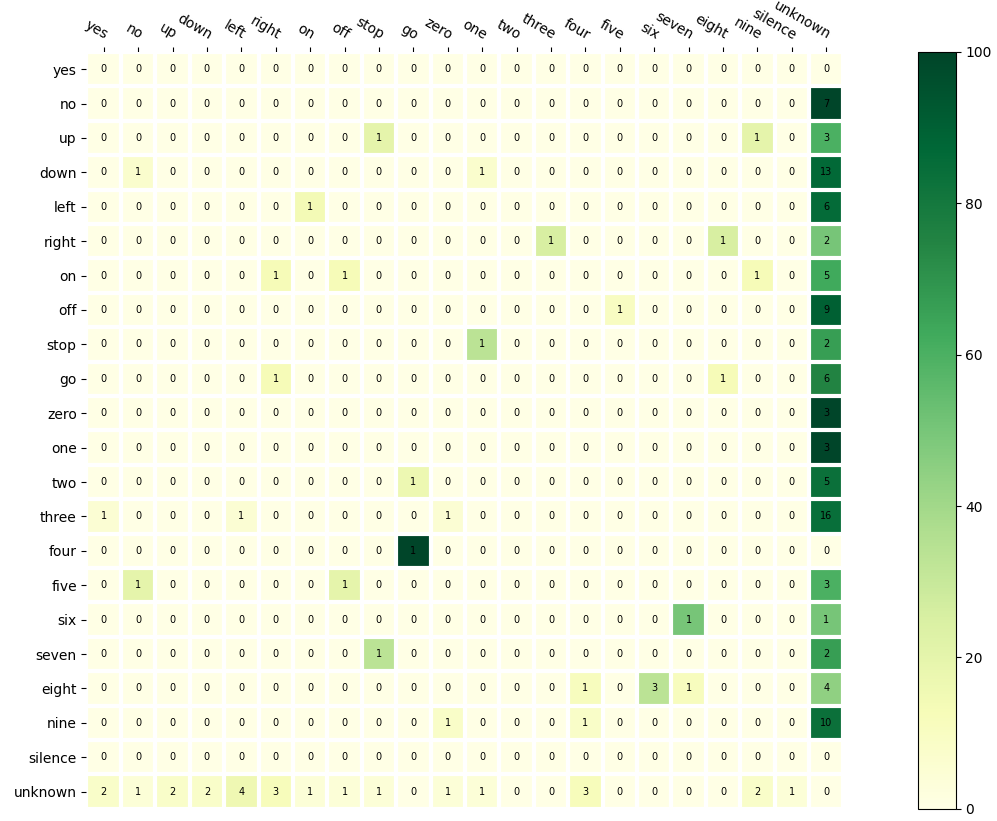
\includegraphics[width=6cm]{chapters/pictures/mlp_mfcc_heatmap.PNG} }}
    \qquad
    \subfloat[\centering SSC preprocessing]{{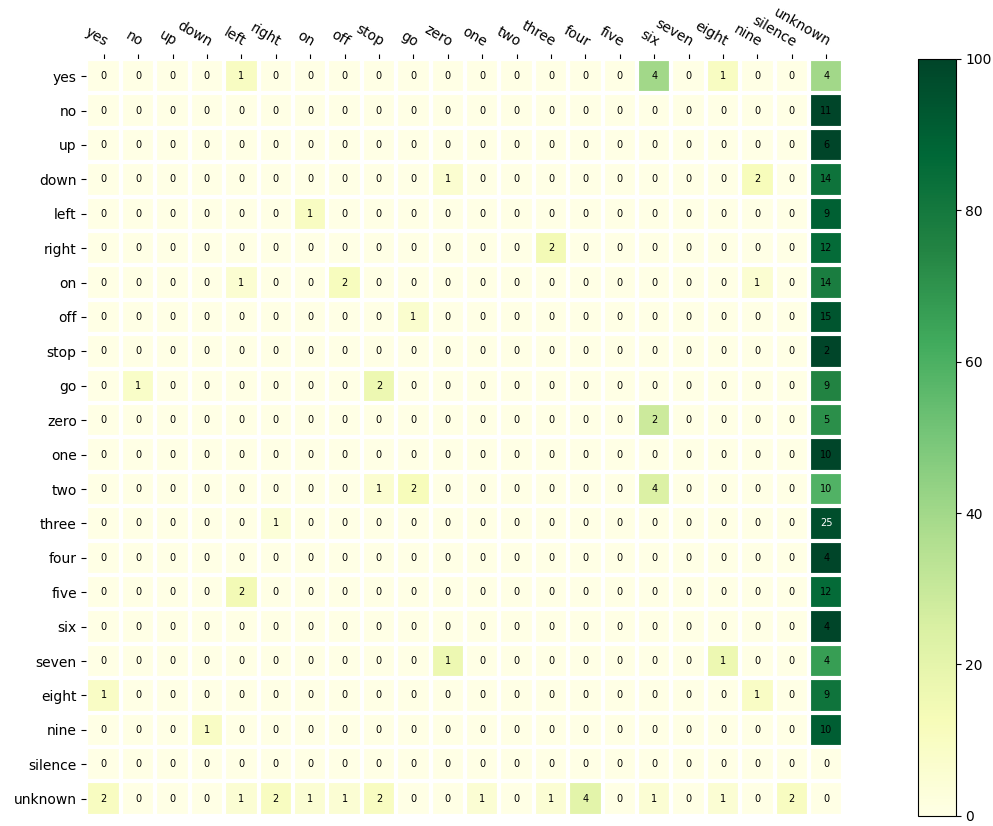
\includegraphics[width=6cm]{chapters/pictures/mlp_ssc_heatmap.PNG} }}
    \caption{Confusion matrix for MLPs with different preprocessing}
    \label{fig:confusion_mlp}

\end{figure}

What we can see is that in general the SSC preprocessing has a classify a lot of out of the ordinary examples in the unknown label. So does the MFCC but with more success.

\newpage

\section{CNN}




From this table \ref{fig:table_cnn} we can see that most of the labels are almost always recognized perfectly with the mfcc preprocessing, but again we see some problems for "three" and "eight". It's even clearer when we look at the heatmap. There is a much higher confusion for "three" than for the others.



\begin{figure}[h!]

    \centering
    \subfloat[\centering MFCC preprocessing]{{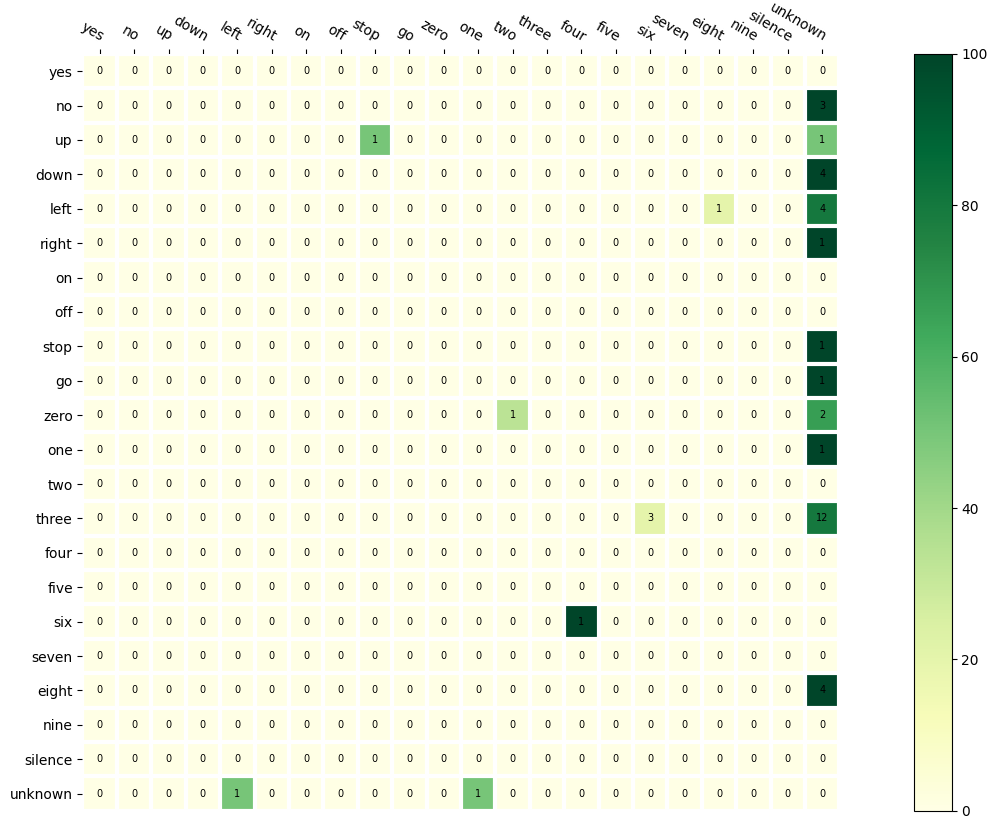
\includegraphics[width=6cm]{chapters/pictures/heatmap_cnn.PNG} }}
    \qquad
    \subfloat[\centering SSC preprocessing]{{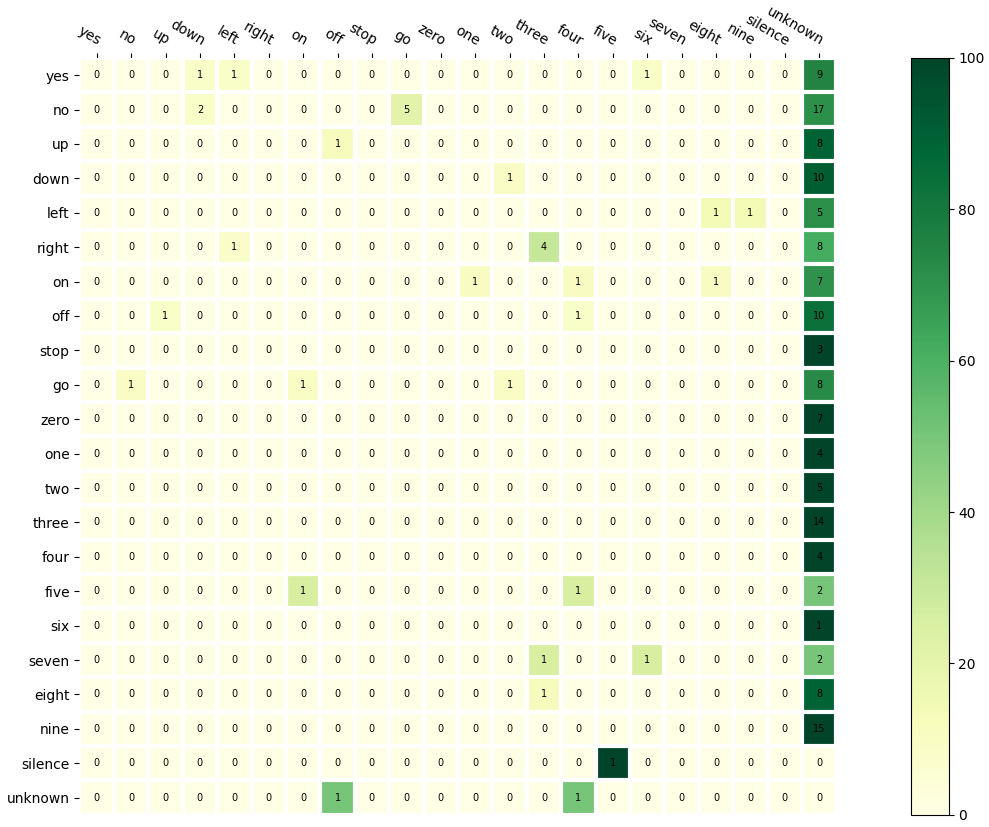
\includegraphics[width=6cm]{chapters/pictures/heatmap_cnn_ssc.PNG} }}
    \caption{Confusion matrix for CNNs with different preprocessing}
    \label{fig:confusion_cnn}

\end{figure}


\newpage



Results for the smaller models are in this table \ref{fig:table_small} .With a smaller model, we can see that "three" is still a problem, so is "nine" but we have a new problematic label emerging which is "no"

\begin{figure}[h!]

    \centering
    \subfloat[\centering MFCC preprocessing]{{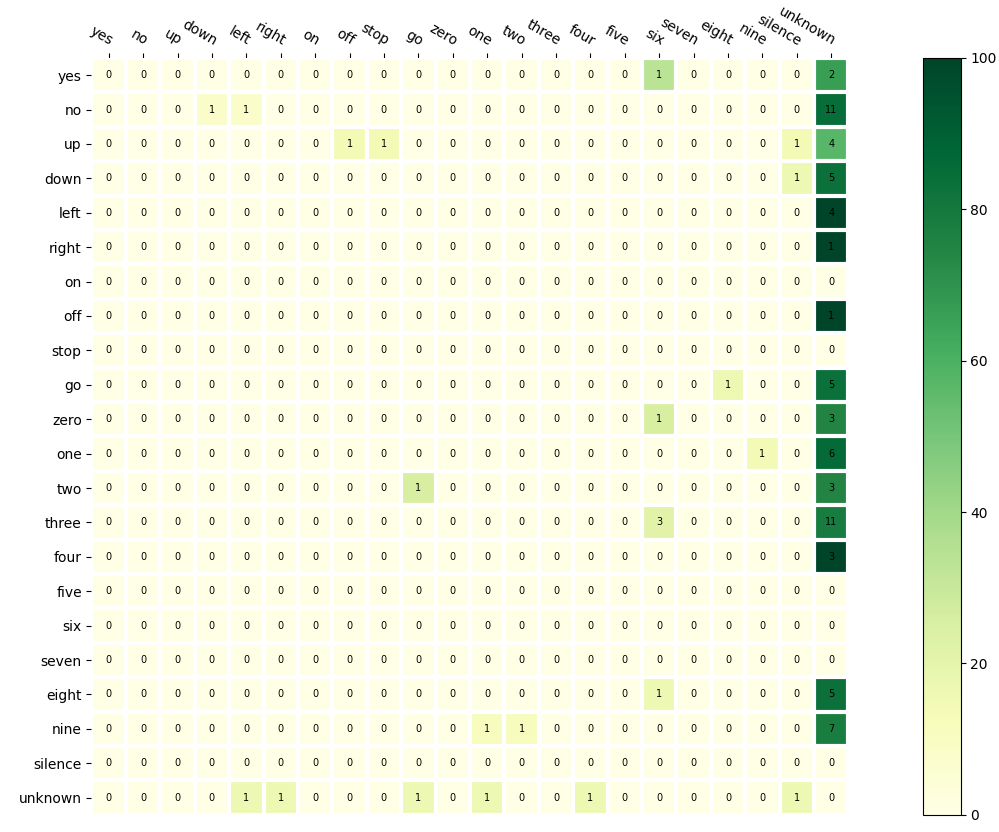
\includegraphics[width=6cm]{chapters/pictures/small_matrixmfcc.PNG} }}
    \qquad
    \subfloat[\centering SSC preprocessing]{{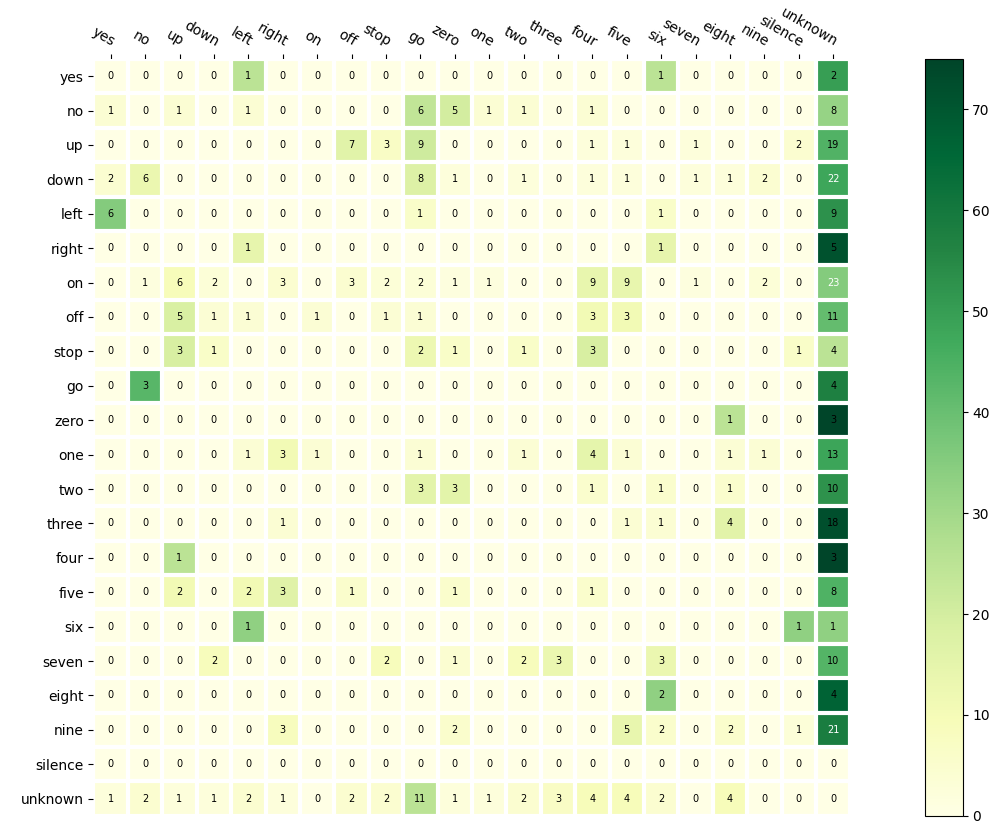
\includegraphics[width=6cm]{chapters/pictures/small_matrix_ssc.PNG} }}
    \caption{Confusion matrix for small CNNs with different preprocessing}
    \label{fig:confusion_small}

\end{figure}


\section{LSTM}




In lstm we can see that the ssc preprocessing is not giving any results. Looks like the structure is not able to learn anything. We didn't plot the heatmap for the ssc preprocessing because there was no point. It's just not accurate at all.

\begin{figure}[h!]
    \centering
    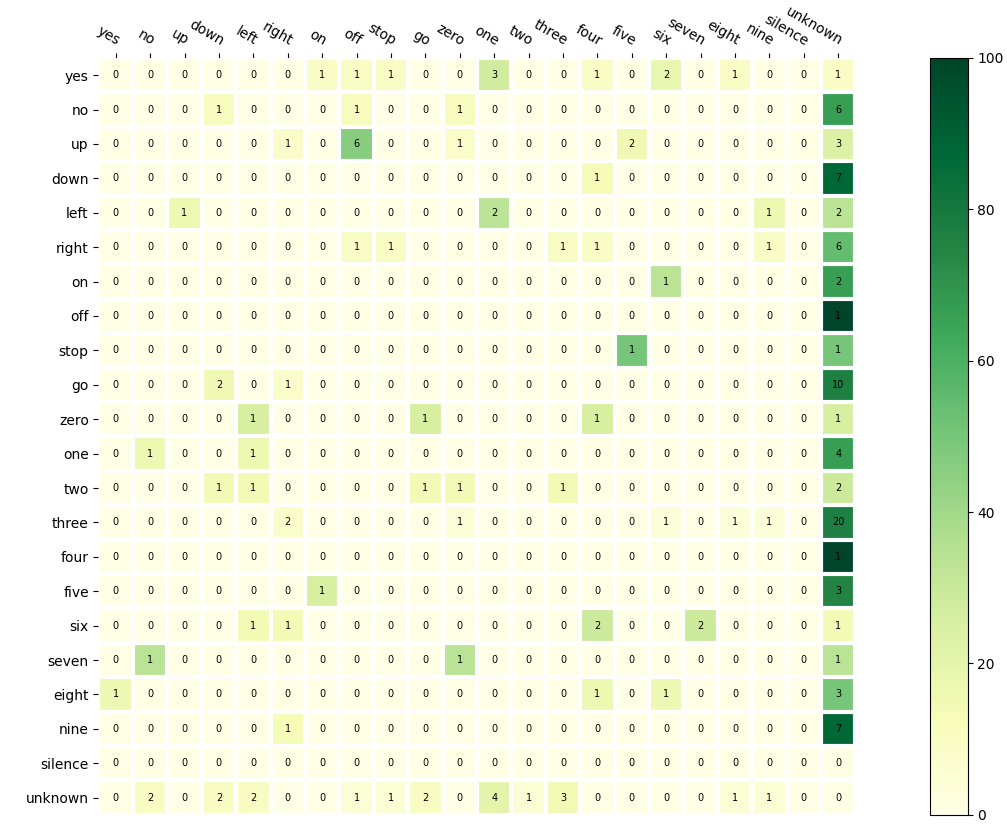
\includegraphics[width=0.5\textwidth]{chapters/pictures/lstm_matrix_mfcc.PNG}
    \caption{Confusions matrix for LSTM and MFCC}
    \label{fig:matrix_lstm_mfcc}
\end{figure}

\newpage

What we can see on the other hand is that the confusions looks like more distributed over the labels. Where usually the only confusions were giving a false unknown label, we have less false positives for the unknown label and more conufusion between regular labels. Still we have a few labels with really inaccurate results like "three".



\begin{figure}[h!]

    \centering
    \subfloat[\centering MFCC preprocessing]{{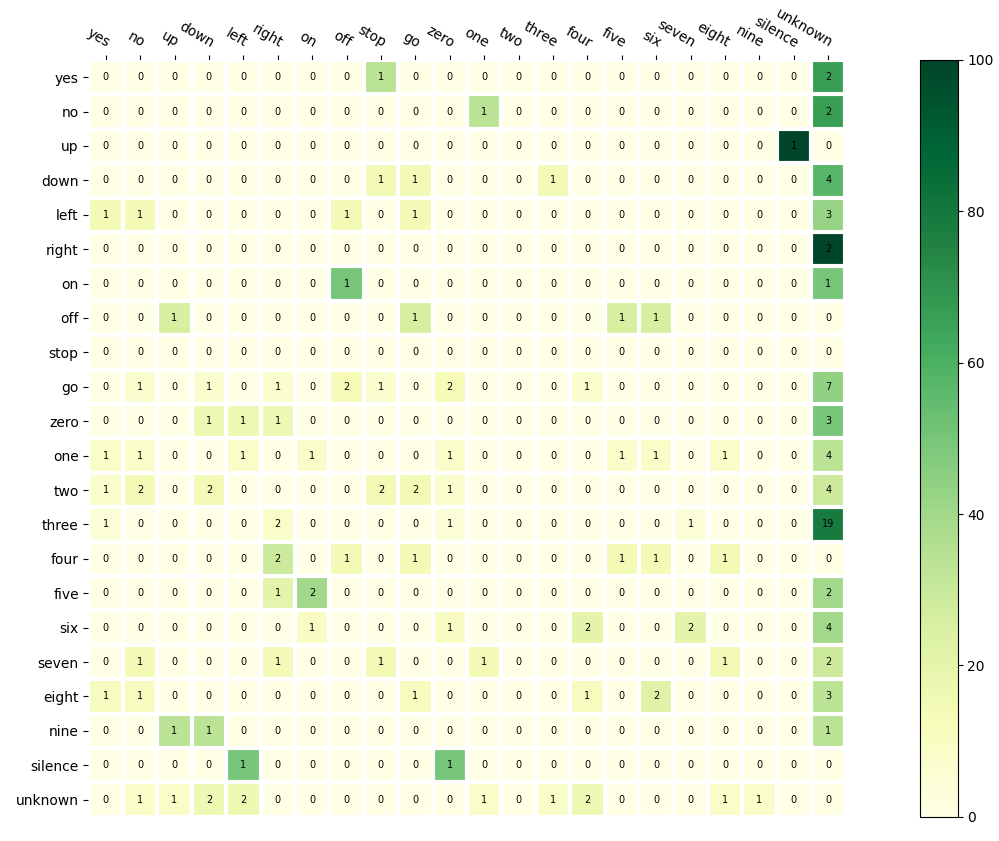
\includegraphics[width=6cm]{chapters/pictures/lstm_cnn_heatmap.PNG} }}
    \qquad
    \subfloat[\centering SSC preprocessing]{{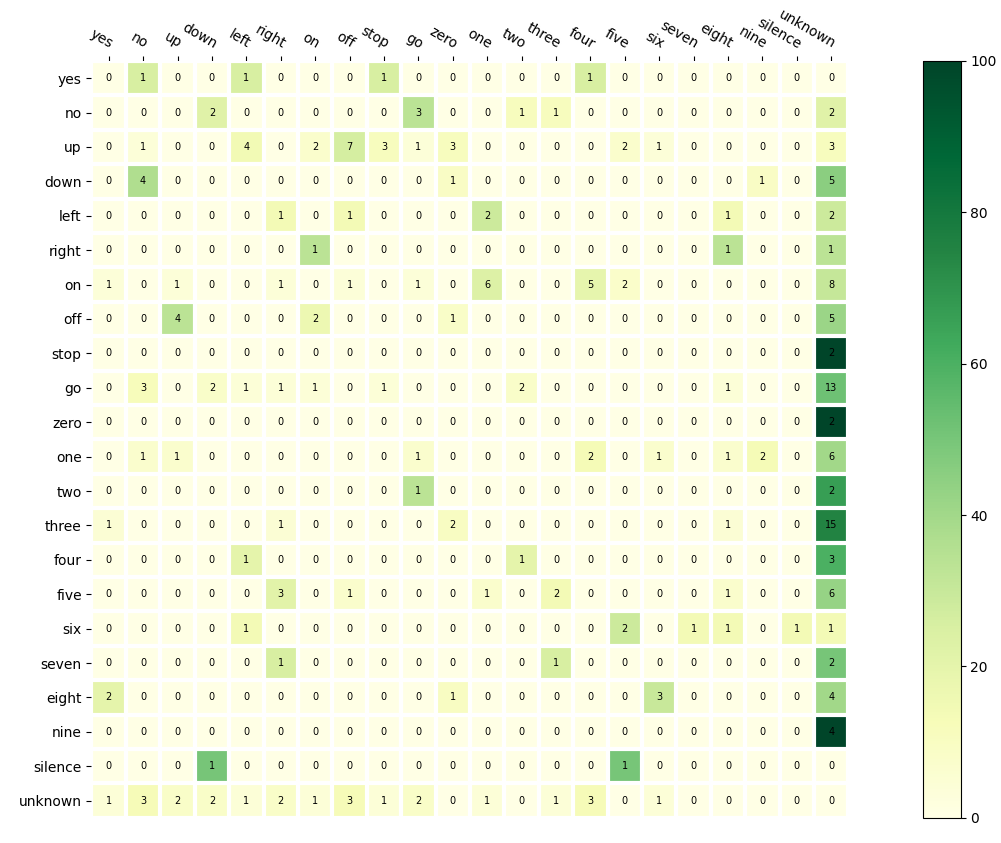
\includegraphics[width=6cm]{chapters/pictures/lstm_cnn_heatmap_ssc.PNG} }}
    \caption{Confusion matrix for LSTM CNN with different preprocessing}
    \label{fig:confusion_lstm_cnn}

\end{figure}

Same results than with the pure lstm in term of distributions of inaccuracies. But we solved the issue of the ssc preprocessing by adding a convolutionnal layer before hand.



\section{Conclusion}

To conclude, we have a few problematic labels, mostly "three". It makes sense since "tree" is present as an unknown word. The differenciation between those two words in the english language is mostly done with the context of the phrase. Here, there is no context. We think that a human would make a significant amount of mistakes if he tried to do the same. We can also see that CNNs and MLPs are classifying more often a word as an unkwown word where lstm are making more mistakes by classifying one known label with another. It would mean that for the CNNs and MLPs, the "templates" created when the model learns are more strict. Therefore when one example is out of the ordinary, it's is classified as an unknown word. While for LSTMs, those templates are more flexible, thus rejecting less words but making more mistakes. We believe that if we were to use one of this network in practice, we would choose a CNN. Because it's better to think that something is unknown than thinking something is true while it's not.